\section[np]{Neyman-Pearson Lemma / Supervised Learning}

\begin{frame}
    \frametitle{Simple example in two dimensions}
    \begin{center}
        \begin{tikzpicture}
            \node[anchor=south west,inner sep=0] (image) at (0,0) {\includegraphics[width=\textwidth]{dataset_orange.png}};
            \onslide<2>{\node[anchor=south west,inner sep=0] (signal) at (4,2.0) {\includegraphics[width=0.5\textwidth]{signal_pdf.png}};
            \begin{scope}[x={(signal.south east)},y={(signal.north west)}]
            	\node[inner sep=0] at (0.4,0.8) {\large{Signal $PDF(\vec{x} | S)$}};
            \end{scope}
			}
            \onslide<3>{\node[anchor=south west,inner sep=0] (background) at (1.8,1.2) {\includegraphics[width=0.6\textwidth]{background_pdf.png}};
            \begin{scope}[x={(background.south east)},y={(background.north west)}]
            	\node[inner sep=0] at (0.4,0.8) {\large{Background $PDF(\vec{x} | B)$}};
            \end{scope}
			}
        \end{tikzpicture}
    \end{center}
\end{frame}

\begin{frame}
    \frametitle{Neyman-Pearson Lemma}
    \begin{center}
        \begin{tikzpicture}
            \node[anchor=south west,inner sep=0] (image) at (0,2) {\includegraphics[width=\textwidth]{npl.png}};
            \node[anchor=south west,inner sep=0] (image) at (0,-0.8) {\Huge{$f(\vec{x}) = \frac{PDF(\vec{x} | S)}{PDF(\vec{x} | B)} = $}};
			      \draw[anchor=south west, thick] (6.8,0) -- (10.6,0);
            \node[anchor=south west,inner sep=0] (image) at (7,0.1) {\includegraphics[width=0.3\textwidth]{signal_pdf.png}};
            \node[anchor=south west,inner sep=0] (image) at (7,-2.1) {\includegraphics[width=0.3\textwidth]{background_pdf.png}};
        \end{tikzpicture}
      \large{Most powerful test at a given significance level to distinguish between two simple hypotheses (signal or background)}
    \end{center}
\end{frame}

\begin{frame}
    \frametitle{Neyman-Pearson Lemma}
    \begin{center}
        \begin{tikzpicture}
            \node[anchor=south west,inner sep=0] (image) at (0,0) {\includegraphics[width=\textwidth]{np_classifier.png}};
        \end{tikzpicture}
    \end{center}
\end{frame}

\begin{frame}
    \frametitle{Neyman-Pearson Lemma}
    \begin{center}
        \begin{tikzpicture}
            \node[anchor=south west,inner sep=0] (image) at (0,0) {\includegraphics[width=\textwidth]{np_statistic.png}};
        \end{tikzpicture}
    \end{center}
\end{frame}

\begin{frame}
    \frametitle{Problem solved? No!}
    \begin{center}
		\begin{itemize}
			\item Howto obtain the signal and background PDFs?
			\begin{itemize}
				\item Usually unknown!
				\item Multiple sources of signal and background
				\item Non gaussian PDF
				\item Nonlinear dependencies among observables
				\item Cannot be sampled in high dimensions (e.g. cannot fill 80-dimensional histogram with enough statistics)
				\item $\rightarrow$ ,,Curse of dimensionality''
			\end{itemize}
		\end{itemize}

        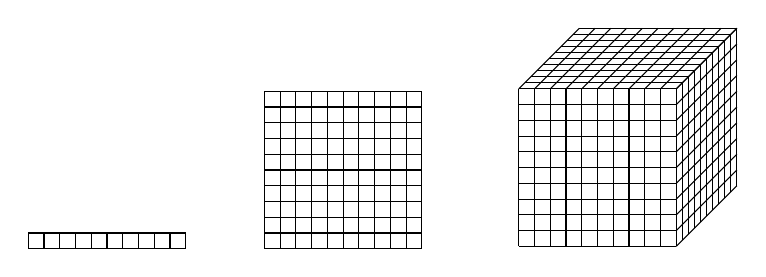
\begin{tikzpicture}
    
        \foreach \x in{0,...,1}
        {   
            \draw (-7,\x*0.2 -0.8) -- (-5,\x*0.2-0.8 );
        }
        \foreach \x in{0,...,10}
        {   
            \draw (\x*0.2-7 ,-0.8) -- (\x*0.2-7 ,-0.6);
        }

        \foreach \x in{0,...,10}
        {   
            \draw (-4,\x*0.2 -0.8) -- (-2,\x*0.2 -0.8 );
            \draw (\x*0.2-4 ,-0.8) -- (\x*0.2-4 , 2-0.8);
        }

        \foreach \x in{0,...,10}
        {   
            \draw (0,\x*0.2 ,2) -- (2,\x*0.2 ,2);
            \draw (\x*0.2 ,0,2) -- (\x*0.2 ,2,2);
            \draw (2,\x*0.2 ,2) -- (2,\x*0.2 ,0);
            \draw (\x*0.2 ,2,2) -- (\x*0.2 ,2,0);
            \draw (2,0,\x*0.2 ) -- (2,2,\x*0.2 );
            \draw (0,2,\x*0.2 ) -- (2,2,\x*0.2 );
        }
        \end{tikzpicture}

    \end{center}
\end{frame}

\begin{frame}
    \frametitle{Solution: Approximate Neyman-Pearson}
	\vspace{-1em}	
	\begin{columns}
	\column{0.6\textwidth}
		\begin{itemize}
			\item Neyman-Pearson Lemma
		\end{itemize}
	\column{0.4\textwidth}
		\vspace{1em}
		\Large{$$f(\vec{x}) = \frac{PDF(\vec{x} | S)}{PDF(\vec{x} | B)}$$}
    \end{columns}
	\vspace{-2em}	
	\begin{columns}
	\column{0.6\textwidth}
		\begin{itemize}
			\item Generative Models
			\begin{itemize}
				\item Analytical approx. (LDA, QDA)
				\item Restricted Boltzmann machine
				\item Kernel density estimator
				\item Gaussian mixture model
			\end{itemize}
		\end{itemize}
	\column{0.4\textwidth}
		\vspace{1em}
		\Large{\begin{align*}f(\vec{x} | S) &\approx PDF(\vec{x} | S) \\ f(\vec{x} | B) &\approx PDF(\vec{x} | B)\end{align*}}
    \end{columns}
	\vspace{-1em}	
	\begin{columns}
	\column{0.6\textwidth}
		\begin{itemize}
			\item Discriminative Models
			\begin{itemize}
				\item (Boosted) Decision Trees
				\item Support Vector Machines
				\item Artificial Neural Networks
			\end{itemize}
		\end{itemize}
	\column{0.4\textwidth}
		\vspace{1em}
		\Large{\begin{align*}f(\vec{x}) &\approx  \frac{PDF(\vec{x} | S)}{PDF(\vec{x} | B)}\end{align*}}
    \end{columns}
\end{frame}

\begin{frame}
    \frametitle{Supervised Learning / How to obtain a model?}

    \vspace{-1em}
    \begin{center}
        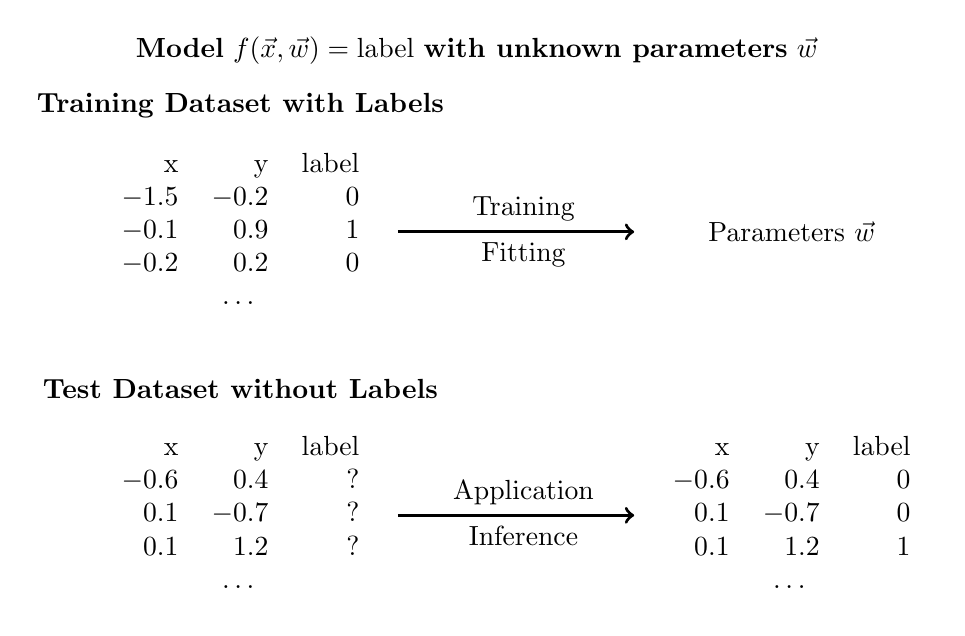
\begin{tikzpicture}[scale=1.0]
            
            \node at (0,2.3) {
                \textbf{Model} $f(\vec{x}, \vec{w}) = \textrm{label}$ \textbf{with unknown parameters} $\vec{w}$
            };
       
            \onslide<2->{
            \node at (-3,1.6) {
                \textbf{Training Dataset with Labels}
            };
            \node at (-3,0) {
                \begin{tabular}{rrr}
                \toprule
                x & y & label \\
                \midrule
                $-1.5$ & $-0.2$ & $0$ \\
                $-0.1$ & $0.9$ & $1$ \\
                $-0.2$ & $0.2$ & $0$ \\
                \multicolumn{3}{c}{\dots} \\
                \bottomrule
                \end{tabular}
            };
            }
        
            \onslide<3->{
            \draw [very thick, ->] (-1,0) -- (2,0)
                    node[above, xshift=-4em] {Training} node[below, xshift=-4em] {Fitting};
            
            \node at (4,0) {Parameters $\vec{w}$};
            }

            \onslide<4->{
            \node at (-3,-2.0) {
                \textbf{Test Dataset without Labels}
            };
            \node at (-3,-3.6) {
                \begin{tabular}{rrr}
                \toprule
                x & y & label \\
                \midrule
                $-0.6$ & $0.4$ & ? \\
                $ 0.1$ & $-0.7$ & ? \\
                $ 0.1$ & $1.2$ & ? \\
                \multicolumn{3}{c}{\dots} \\
                \bottomrule
                \end{tabular}
            };
        }
            \onslide<5->{
            
            \draw [very thick, ->] (-1,-3.6) -- (2,-3.6)
                    node[above, xshift=-4em] {Application} node[below, xshift=-4em] {Inference};
            
            \node at (4,-3.6) {
                \begin{tabular}{rrr}
                \toprule
                x & y & label \\
                \midrule
                $-0.6$ & $0.4$ &  0\\
                $ 0.1$ & $-0.7$ & 0 \\
                $ 0.1$ & $1.2$ & 1 \\
                \multicolumn{3}{c}{\dots} \\
                \bottomrule
                \end{tabular}
            };
        }

        \end{tikzpicture}
    \end{center}

\end{frame}


\begin{frame}
    \frametitle{Example: Linear Model}
    \begin{align*}
    f(\vec{x}, \vec{w}) &= \vec{x} \cdot \vec{w}
    \end{align*}
    \begin{center}
        \begin{tikzpicture}
            \node[anchor=center,inner sep=0] (image) at (0,0) {\includegraphics[width=0.8\textwidth]{dataset_orange.png}};
           \onslide<2-3>{
             \draw[name path=A, line width=0.05 cm] (0,2.3) -- (0, -2.3);
             \node at (0,2.6) {$\vec{w} = (0, 1)\quad$ ?};
			}
          \onslide<3>{
            \draw [name path=B1] plot [smooth] coordinates {(0,2) (-1.5,0.8) (-0.5,0) (-1,-1) (0,-2)};
            \tikzfillbetween[of=A and B1] {fill=blue,fill opacity=0.4};
            \draw [name path=B2] plot [smooth] coordinates {(0,2) (0.7,1.0) (0.6,0) (1,-0.5) (0,-2)};
            \tikzfillbetween[of=A and B2] {fill=orange,fill opacity=0.4};
		   }
           \onslide<4-5>{
             \draw[name path=C, line width=0.05 cm] (-3,-0.5) -- (3, 0.5);
             \node at (0,2.6) {$\vec{w} = (6, 1)\quad$ !};
			}
         \onslide<5>{
           \draw [name path=D1] plot [smooth] coordinates {(-3,-0.5) (-1,1.5) (0,0.5) (1,0.3) (3,0.5)};
           \tikzfillbetween[of=C and D1] {fill=blue,fill opacity=0.4};
           \draw [name path=D2] plot [smooth] coordinates {(-3,-0.5) (-1,-0.3) (0,-0.5) (1,-1.5) (3,0.5)};
           \tikzfillbetween[of=C and D2] {fill=orange,fill opacity=0.4};
	   }
        \end{tikzpicture}
    \end{center}
\end{frame}

\begin{frame}
    \frametitle{More Questions}
    \begin{center}
		\begin{itemize}
      \item \textbf{How to obtain training data required for these models?}
			\begin{itemize}
				\item In industry usually historical data ($\rightarrow$ time-series)
				\item In HEP usually simulated data ($\rightarrow$ systematics)	
				\item Sometimes we can use real data ($\rightarrow$ data-driven techniques)
			\end{itemize}
    \item \textbf{How to train, optimize and evaluate the quality of the models and compare them?}
			\begin{itemize}
				\item Train model on training data ($\rightarrow$ regularization techniques)
				\item Optimize model on validation data ($\rightarrow$ hyper-parameter optimization)
				\item Test model on test data ($\rightarrow$ ROC curves)
				\item Apply model on unlabeled data ($\rightarrow$ systematics)
			\end{itemize}
		\end{itemize}
    \end{center}
\end{frame}

\begin{frame}
    \frametitle{Classification Quality}

    \begin{center}

      \begin{itemize}
        \item Misclassification Rate (= Fraction of wrongly classifier events)
        \item Type I Error (= False Positive Rate)
        \item Type II Error (= 1 - True Positive Rate)
      \end{itemize}
      \vspace{1em}
        \textbf{Problem: Depends on the chosen cut on the classifier output!}
    \end{center}
\end{frame}

\begin{frame}
    \frametitle{Classification Quality}
    \textbf{Solution: Receiver operating characteristic}\\
     {\small Visualizes the false positive rate (fpr) as a function of the true positive rate (tpr)}\\
     \vspace*{1em}

     \textbf{More General}\\
     {\small Visualizes two mutually exclusive objectives as a curve in a plane}\\
     \begin{center} 
     \includegraphics[width=0.5\textwidth]{np_roc.png}
     \end{center}
\end{frame}

\begin{frame}
    \frametitle{Classification Quality}
    \begin{center}
        \begin{tikzpicture}
            \onslide<1>{\node[anchor=south west,inner sep=0] (image) at (0,0) {\includegraphics[width=\textwidth]{np_statistic.png}};}
            \onslide<2>{\node[anchor=south west,inner sep=0] (image) at (0,0) {\includegraphics[width=\textwidth]{np_statistic_cut.png}};}
            \onslide<3>{\node[anchor=south west,inner sep=0] (image) at (0,0) {\includegraphics[width=\textwidth]{np_statistic_cut_zoomed.png}};}
            \onslide<4>{\node[anchor=south west,inner sep=0] (image) at (0,0) {\includegraphics[width=\textwidth]{np_roc.png}};}
            \onslide<5>{\node[anchor=south west,inner sep=0] (image) at (0,0) {\includegraphics[width=\textwidth]{np_roc_shaded.png}};}
            \onslide<5>{\node at (6, 3) {\large{Allowed Region for an arbitrary classifier}};}
        \end{tikzpicture}
    \end{center}
\end{frame}
